\documentclass[cic,tc]{iiufrgs}
\usepackage[utf8]{inputenc}   % pacote para acentuação
\usepackage{graphicx}         % pacote para importar figuras
\usepackage{times}            % pacote para usar fonte Adobe Times
\usepackage{algpseudocode}
\usepackage{url}
\usepackage{amsmath}
% \usepackage{palatino}
% \usepackage{mathptmx}       % p/ usar fonte Adobe Times nas fórmulas
\usepackage[alf,abnt-emphasize=bf]{abntex2cite}	% pacote para usar citações abnt

%
% Informações gerais
%
\title{Estudo e otimização dos softwares de bioinformática do Hospital de
Clínicas de Porto Alegre}

\author{Farah}{Alef}

% orientador e co-orientador são opcionais (não diga isso pra eles :))
\advisor[Prof.~Dr.]{Geyer}{Claudio Fernando Resin}
\coadvisor[Prof.~Dr.]{Anjos}{Julio Cesar Santos}

% a data deve ser a da defesa; se nao especificada, são gerados
% mes e ano correntes
\date{novembro}{2021}

% o local de realização do trabalho pode ser especificado (ex. para TCs)
% com o comando \location:
\location{Porto Alegre}{RS}

% itens individuais da nominata podem ser redefinidos com os comandos
%
% palavras-chave
% iniciar todas com letras minúsculas, exceto no caso de abreviaturas
%
\keyword{bioinformática}
\keyword{paralelismo}
\keyword{codeml}
\keyword{PAML}
\keyword{SAMtools}
%\keyword{}

%\settowidth{\seclen}{1.10~}

\begin{document}

% folha de rosto
% às vezes é necessário redefinir algum comando logo antes de produzir
% a folha de rosto:
% \renewcommand{\coordname}{Coordenadora do Curso}
\maketitle

% dedicatoria
% \clearpage
% \begin{flushright}
%     \mbox{}\vfill
%     {\sffamily\itshape
%       ``If I have seen farther than others,\\
%       it is because I stood on the shoulders of giants.''\\}
%     --- \textsc{Sir~Isaac Newton}
% \end{flushright}

% agradecimentos
%\chapter*{Agradecimentos}
%Agradeço ao \LaTeX\ por não ter vírus de macro\ldots

% resumo na língua do documento
\begin{abstract}
  Neste trabalho foi realizado um estudo e otimização dos problemas de
  desempenho presentes em alguns dos softwares de bioinformática utilizados
  pelo grupo de pesquisa em genética do Hospital de Clínicas de Porto Alegre
  (HCPA), empregando para isso técnicas de processamento paralelo. O trabalho
  focou no software de análise filogenética codeml, do pacote PAML, amplamente
  utilizado na literatura, e no software SAMtools, usado para chamada de
  variantes, igualmente popular. Foi desenvolvida uma ferramenta de
  paralelização de \textit{jobs} do SAMtools, reduzido de vários dias para
  poucas horas o tempo de análise do grupo de pesquisa, enquanto que no caso do
  codeml foi realizado uma análise de desempenho de alternativas encontradas em
  revisão bibliográfica, fornecendo aos pesquisadores uma ferramenta que reduz
  em mais da metade o tempo de execução em relação ao codeml original.
  \end{abstract}

% resumo na outra língua
% como parametros devem ser passados o titulo e as palavras-chave
% na outra língua, separadas por vírgulas
\begin{englishabstract}{Study and optimization of the bioinformatics software used by Hospital de Clínicas de Porto Alegre}{Bioinformatics, parallelism, codeml, PAML, SAMtools} In this paper we studied and optimized the performance bottlenecks found in some of the bioinformatics software used by the genetics research group from Hospital de Clínicas de Porto Alegre (HCPA), employing parallel programming techniques to achieve these goals. The focus of our work was in the phylogenetic analysis software called codeml, from the PAML package, which is widely used in the literature, as well on the SAMtools software, used for variant calling, also popular. We developed a tool for the parallel execution of SAMtools jobs, reducing total execution time for the group's input from various days to a few hours, while in the case of codeml we analyzed the performance of solutions found in a bibliography review, supplying the researches with a tool whose execution time is half that of codeml.
\end{englishabstract}

% lista de figuras
\listoffigures

% lista de tabelas
\listoftables

% lista de abreviaturas e siglas
% o parametro deve ser a abreviatura mais longa
\begin{listofabbrv}{POSIX}
    \item[POSIX] \textit{Portable Operating System Interface}
    \item[HCPA] Hospital de Clínicas de Porto Alegre
    \item[GATK] \textit{Genome Analysis Toolkit}
    \item[PAML] \textit{Phylogenetic Analysis By Maximum Likelihood}
    \item[NCBI] \textit{National Center for Biotechnology}
    \item[BFGS] Broyden–Fletcher–Goldfarb–Shanno
    \item[CPU] \textit{Central Processing Unit}
    \item[GPU] \textit{Graphics Processing Unit}
    \item[API] \textit{Application Programming Interface}
    \item[DNA] Ácido desoxirribonucleico
    \item[RNA] Ácido ribonucleico
    \item[RAM] \textit{Random access memory}
    \item[ARC] \textit{Advanced Resource Connector}
    \item[PBS] \textit{Population Branch Statistic}
    \item[GRC] \textit{Genome Reference Consortium}
    \item[IPC] \textit{Inter process communication}
    \item[SNV] \textit{Single-nucleotide variant}
    \item[JIT] \textit{Just-in-time}
    \item[GHz] Giga hertz
    \item[GB] Giga byte
    \item[TB] Tera byte
    \item[IO] \textit{Input output}
\end{listofabbrv}

% idem para a lista de símbolos
\begin{listofsymbols}{$F_{ST}$}
    \item[$\omega$] Taxa de substituição
    \item[$dN$] Substituições não-sinônimas
    \item[$dS$] Substituições sinônimas
    \item[$F_{ST}$] Índice de fixação
    \item[$\frac{\partial f}{\partial x_i}$] Derivada parcial de $f$ com respeito a $x_i$
\end{listofsymbols}

% Sumário
\tableofcontents

%
%
% Introdução
%
%

\chapter{Introdução}

%
% Breve contexto do problema
%
O grupo de pesquisa em genética do Hospital de Clínicas de Porto Alegre (HCPA)
utiliza uma série de softwares de bioinformática para análise de sequências
genéticas. Alguns desses softwares apresentam problemas de desempenho, como
tempo de execução ou uso de memória proibitivamente elevados, o que dificulta
ou impede suas análises.

Nomeadamente, para a análise filogenética, que visa elucidar eventos evolutivos
na linhagem dos seres vivos, o grupo emprega o software codeml, do pacote
PAML.\cite{yang2007paml} Apesar de amplamente utilizado na literatura e
considerado referência para análise filogenética,\cite{maldonado2016lmap} o
codeml possui implementação ingênua de métodos numéricos computacionalmente
custosos.\cite{yang2020paml} Para uma única entrada dos pesquisadores, são
necessárias mais de 16 horas de processamento em hardware moderno.

Já para a execução da chamada de variantes, processo que visa identificar
variações entre sequências genéticas alinhadas, o grupo emprega os pacotes
SAMtools \cite{li2009sequence} ou ANGSD \cite{korneliussen2014angsd}, aquele
sendo considerado estado da
arte.\cite{poplin2018universal}\cite{yao2020evaluation} O pacote SAMtools,
amplamente utilizado na literatura para manipulação de arquivos de sequências
genéticas alinhadas, \cite{danecek2021twelve} apresenta tempo de execução
demasiadamente elevado. Para uma entrada consistindo de apenas oito amostras,
são necessários mais de quatro dias de processamento em um hardware moderno.
Enquanto isso, o pacote ANGSD apresenta uso de memória proibitivamente elevado.
Para uma entrada consistindo de apenas seis amostras, o uso de memória
ultrapassava os 64 GB.


%
% Motivação e Objetivos (alto nível)
%
Motivado pela resolução dos problemas de desempenho enfrentados pelos
pesquisadores do HCPA mesmo com ferramentas consideradas estado da arte, este
trabalho objetivou o estudo desses softwares e de seus gargalos de desempenho,
visando seu mapeamento e resolução. Partindo da observação que esses softwares
não empregam técnicas de processamento paralelo ou o fazem de forma limitada,
objetivou-se o desenvolvimento de um ferramental que empregue tais técnicas, a
fim de beneficiar-se de ambientes multiprocessados, ubíquo em hardware moderno.

Para isso, planejou-se uma revisão bibliográfica a respeito dos softwares de
análise filogenética e chamada de variantes, seguida de análises de desempenho
dos softwares encontrados frente àqueles atualmente utilizados no HCPA. A
seguir, objetivou-se o traço de perfis de execução das ferramentas estudadas,
visando identificar seus gargalos de processamento e estudar a possibilidade de
desenvolvimento de novas ferramentas que os eliminem, potencialmente através da
execução paralela dos algoritmos empregados.

%
% Contribuções
%
\section{Contribuições}

Neste trabalho foram mapeados e solucionados os problemas de uso de memória e
tempo de execução proibitivamente altos enfrentados pelos pesquisadores do HCPA.
Através de análises de desempenho e desenvolvimento de uma nova ferramenta que
aplica técnicas de processamento paralelo, foi reduzido em até 91,63\% o tempo
de processamento dos pipelines de análise executados no HCPA.

% TODO confirmar e pegar o tempo exato
No caso dos softwares de análise filogenética, para o qual emprega-se o pacote
PAML no HCPA, a identificação de softwares alternativos através de um estudo da
literatura, aliado ao desenvolvimento de uma ferramenta para sua execução
paralela, resultou na redução de mais da metade do tempo de execução, para as
entradas utilizadas pelos pesquisadores.

Já no caso do processo de chamada de variantes, para o qual empregam-se os
pacotes ANGSD ou SAMtools no HCPA, foi desenvolvida uma ferramenta para
execução paralela desse que reduziu em 91,63\% o tempo de execução em relação
ao pipeline originalmente utilizado pelos pesquisadores, ao mesmo tempo
evitando problemas de alto uso de memória como aqueles presentes no pacote
ANGSD. Isso permitiu que o SAMtools fosse utilizado como alternativa definitiva
ao software ANGSD, cujos problemas de desempenho foram mapeados através de um
perfil de execução, mas não foram atacados nesse trabalho, sendo a ferramenta
de paralelização do SAMtools a alternativa favorecida.

Além disso, a ferramenta desenvolvida nesse trabalho evita deficiências
presentes em outros trabalhos que visam melhorar o desempenho do SAMtools, que
é considerado estado da arte. Por exemplo, a ferramenta desenvolvida apresenta
baixo uso de memória, em contraste com alternativas encontradas na literatura
como PVCtools e elPrep, e possui, diferente de aplicações publicadas na
literatura como sambamba e elPrep, suporte a formatos de arquivos mais modernos
utilizados pelos pesquisadores do HCPA.

%
% Organização das outras seções
%
\section{Estrutura do texto}

O resto do texto está organizado da seguinte maneira: no capítulo
\ref{chap:background} é apresentado um background de bioinformática relevante à
compreensão desse trabalho, detalhando as áreas de estudo do grupo de pesquisa
em genética, os softwares empregados no HCPA, e os formatos de arquivo
envolvidos. No capítulo \ref{chap:anteriores} é apresentado o estado da arte
para cada área de estudo, bem como trabalhos relacionados a tais softwares. Já
no capítulo \ref{chap:mod} é apresentada a metodologia de avaliação, enquanto
que no capítulo \ref{chap:imp} apresenta-se sua implementação e os resultados
obtidos.  Por fim, no capítulo \ref{chap:conc} é apresentada uma conclusão,
seguida das referências.

%
%
% Background
%
%

\chapter{Background}
\label{chap:background}

Neste capítulo são introduzidos conceitos de bioinformática necessários à
compreensão dos softwares que foram objeto de estudo desse trabalho.
Na seção \ref{sec:filo} é apresentado o conceito de análise filogenética,
objeto de estudo dos usuários do pacote PAML; na seção \ref{sec:call} é exposto
o conceito chamada de variantes, para o qual os pacotes ANGSD e SAMtools
são empregados, e na seção \ref{sec:formats} são descritos os formatos de
arquivos utilizados para cada um desses processos, relevantes ao entendimento
das soluções desenvolvidas.

\section{Análise filogenética}
\label{sec:filo}

A análise filogenética compreende o estudo da evolução de um ou mais organismos
e suas características. O grupo de pesquisa em genética do HCPA realiza tal
estudo a nível molecular, isto é, através da análise das sequências genéticas
de diferentes linhagens evolutivas de uma espécie ou grupo de espécies.

As sequências genéticas em questão são representações da informação genética
dos seres vivos. Em termos simples, trata-se da sequência de códons (triplas de
nucleotídeos) que, encadeados em hélice dupla, formam o DNA dos seres vivos e o
RNA produzido a partir dele. Cada códon que compõem a sequência genética
determina um aminoácido específico a ser produzido na síntese proteica.

O alfabeto (código) genético é composto de apenas quatro tipos de nucleotídeos:
adenina (A), guanina (G), uracila (U), e citosina (C). Como os códons são
constituídos sempre de três nucleotídeos, existem $4^3 = 64$ códons distintos,
dos quais três são códons de terminação, que indicam o fim da etapa de tradução
na síntese proteica, enquanto os outros 61 códons traduzem para um aminoácido
específico.

Já as proteínas são compostas por apenas 20 aminoácidos distintos. Sendo assim,
a maioria dos aminoácidos é traduzido por mais de um códon. Em outras palavras,
a substituição de certos códons no DNA não produz alteração nos aminoácidos
gerados na síntese proteica.

As substituições que não geram alterações na síntese proteica são chamadas de
sinônimas ou silenciosas, enquanto as que modificam os aminoácidos gerados são
não sinônimas. Acredita-se que as substituições sinônimas sejam mais comuns e
não sofram tanta pressão seletiva. A taxa de substituições sinônimas e não
sinônimas $\omega = \frac{dN}{dS}$ é, assim, uma medida de seleção natural,
conforme a tabela \ref{tbl:ex1}.\cite{yang2002codon}

\begin{table}[h]
    \caption{Taxas de substituição}
    \centering
        \begin{tabular}{c|c}
          \hline
          \textit{Taxa}  &   \textit{Seleção} \\
          \hline
          \hline
          $\omega = 1$ & Seleção neutra \\
          $\omega < 1$ & Seleção negativa ou purificadora \\
          $\omega > 1$ & Seleção positiva \\
          \hline
        \end{tabular}
      \legend{Fonte: \cite{yang2002codon}}
    \label{tbl:ex1}
\end{table}

O propósito de softwares de análise filogenética como o pacote PAML é, em
síntese, detectar eventos de seleção positiva nas diferentes linhagens da
árvore filogenética de uma espécie. Para isso, o PAML utiliza modelos
estatísticos de máxima verossimilhança para comparar a hipótese de ocorrência
desses eventos contra a hipótese nula de seleção neutra ou
negativa.\cite{moretti2012gcodeml}

\section{Chamada de variantes}
\label{sec:call}

A chamada de variantes consiste em uma série de métodos para identificação de
variações entre sequências genéticas.\cite{nielsen2011genotype} Um dos
objetivos dessa identificação é a compreensão das causas de variações
fenotípicas observadas entre diferentes populações de uma espécie, através do
estudo a nível molecular das variações genéticas entre indivíduos dessas
populações.\cite{jiang2019population} Em particular, a chamada de variantes de
nucleotídeo único (\textit{SNV calling}) identifica variações na estrutura
genética a nível de um único nucleotídeo.\cite{khurana2016role}

Essas sequências genéticas sendo comparadas podem apresentar erros de leitura,
provenientes de um processo complexo com múltiplas etapas propensas a falhas.
Por exemplo, os próprios instrumentos utilizados possuem propriedades físicas
que geram leituras imperfeitas. A chamada de variantes emprega diferentes
métodos para identificar não apenas as diferenças entre as sequências
analisadas, mas também distinguir as diferenças reais daquelas causadas por
erros de leitura.\cite{poplin2018universal} Dependendo dos métodos e
ferramentas empregados para chamada de variantes, os resultados obtidos são
diferentes e muitas vezes complementares entre
si.\cite{hwang2015systematic}\cite{gezsi2015variantmetacaller}\cite{guo2015seqmule}

Em particular, cada método de chamada de variantes possui resultados mais ou
menos robustos dependendo do método de leitura das sequências analisadas, visto
que o pipeline de filtragem empregado na chamada de variantes é muitas vezes
afinado para tecnologias de leitura específicas.\cite{poplin2018universal} Um
dos pacotes utilizados para realizar a chamada de variantes é o
SAMtools,\cite{pirooznia2014validation} sendo considerado robusto e estado da
arte junto ao software
GATK,\cite{crysnanto2019accurate}\cite{hwang2015systematic}\cite{yao2020evaluation}\cite{poplin2018universal}
que é descrito em mais detalhes na seção \ref{sec:alt}.

Uma vez identificadas as variantes, é necessário ainda uma análise da sua
responsabilidade nas diferenças fenotípicas observadas entre os indivíduos sob
estudo. Para isso são comparadas métricas de diferenciação da estrutura
genética dos indivíduos sob análise. Uma métrica de diferença na estrutura
genética entre duas populações de uma espécie é o índice de fixação ou
$F_{ST}$, baseado, em suma, na variança da frequência alélica das duas
populações -- a frequência alélica sendo a frequência relativa com a qual um
alelo (variante de um gene) ocorre. Genes com um $F_{ST}$ alto são potenciais
alvos de seleção natural.\cite{yi2010sequencing}

Como o $F_{ST}$ é uma métrica de comparação de pares, ele não é capaz de
identificar a direção das mudanças, nem pode ser utilizado como única métrica
para identificar eventos de seleção natural. O \textit{Population Branch
Statistic} ou PBS consiste de um método estatístico que utiliza comparações em
pares do $F_{ST}$ entre três populações distintas para quantificar as
diferenças entre suas sequências genéticas. Genes com valor PBS alto indicam
seleção positiva.\cite{jiang2019population} Uma descrição mais aprofundada do
método foge ao escopo desse trabalho, e pode ser encontrada em
\cite{yi2010sequencing}. O software ANGSD é um dos pacotes que podem ser
empregados para execução do método PBS.

Os pesquisadores do HCPA utilizam os pacotes ANGSD ou SAMtools para realizar a
chamada de variantes visando entender variações fenotípicas entre populações
humanas, utilizando para isso o método PBS através do software ANGSD ou através
de um pipeline utilizando o SAMtools e posterior análise estatística das
saídas.

\section{Formatos de arquivos}
\label{sec:formats}

% TODO aqui tem bastante espaço para engordar o texto entrando em mais detalhes
% sobre os formatos de arquivos

Fundamental ao entendimento de algumas otimizações realizadas nesse trabalho é
um conhecimento básico dos diferentes formatos de arquivo utilizados para
armazenamento de informação genética, no campo da bioinformática. Neste
trabalho foram trabalhados com arquivos nos formatos SAM, BAM, CRAM, BCF, VCF,
FASTA, e NWK, descritos brevemente nesta seção.

Os formatos SAM, BAM, e CRAM, representam sequências genéticas alinhadas a um
genoma de referência. O formato SAM traz uma representação em texto plano, o
BAM é seu equivalente binário, e o CRAM é uma versão binária com compressão.
Tais arquivos podem ser manipulados com a ferramenta samtools, do pacote
SAMtools.\cite{danecek2021twelve} Amostras de sequências genéticas de
indivíduos da espécie humana são fornecidos no formato CRAM pelo projeto 1000
Genomes, um esforço colaborativo internacional que visa sequenciar o genoma
humano e disponibilizar a informação publicamente.\cite{via20101000}

A chamada de variantes realiza comparações entre múltiplos arquivos nos
formatos supracitados, produzindo arquivos que representam as variantes
encontradas. Quando as informações de variantes são armazenadas em texto plano
diz-se do arquivo VCF, seu equivalente binário sendo o formato BCF, ambos
gerados e manipulados pela ferramenta bcftools, do pacote
SAMtools.\cite{danecek2021twelve}

Já o formato FASTA é utilizado para representar sequências
de nucleotídeos ou aminoácidos. Introduzido pela primeira vez em
\cite{fasta}, é hoje ubíquo no campo da
bioinformática.\cite{shen2016seqkit} Os genomas de referência aos quais as
demais sequências genéticas são alinhadas são fornecidos nesse formato, e o
pacote SAMtools providencia ferramental para manipulação desses arquivos. O
genoma de referência é publicado pelo órgão \textit{Genome Reference
Consortium} (GRC), e a publicação mais atual é nomeada GRCh38, de
2013.\cite{GUO201783} Convém mencionar que o software PAML também recebe
arquivos nesse formato como entrada.

O projeto 1000 Genomes fornece ainda sequências alinhadas ao genoma de
referência anterior, GRCh37, no formato BAM, consideravelmente maior que o
CRAM. Esses arquivos, diferente dos mais recentes no formato CRAM e alinhados
ao GRCh38, encontram-se disponíveis em \textit{mirrors} como do
\textit{National Center for Biotechnology} (NCBI), providenciando maior largura
de banda.\cite{clarke20121000}

Por fim, para o software PAML, além de arquivos FASTA contendo as sequências
genéticas dos indivíduos da árvore filogenética, a árvore em si consiste de uma
das entradas do software. A árvore é fornecida no formato NWK ou Newick, um
formato texto plano com representação flexível, que basicamente separa os nodos
por vírgula e utiliza parênteses para distinguir nodos internos de folhas.
Originalmente introduzido na aplicação PHYLIP \cite{felsenstein1993phylip}, é
amplamente utilizado para representação de árvores filogenéticas.\cite{fredslund2006phy}

%
%
% Trabalhos relacionados / Estado da arte
%
%

\chapter{Trabalhos relacionados}
\label{chap:anteriores}

Nesta seção é apresentado o estado da arte nas áreas de análise filogenética e
chamada de variantes, bem como trabalhos relacionados aos softwares utilizados
pelos pesquisadores do HCPA -- codeml, do pacote PAML, ANGSD, e SAMtools.

\section{Análise filogenética}

A implementação de referência ou \textit{gold standard} na área de análise
filogenética é a aplicação codeml, do pacote PAML.\cite{valle2014optimization}
Em suma, o codeml detecta eventos de seleção utilizando diferentes modelos de
variação das taxas de substituição $\omega$ ao longo da sequência genética
(\textit{site models} ou modelos de sítio) e das linhagens da árvore
filogenética (\textit{branch models} ou modelos de linhagem). Métodos
estatísticos de máxima verossimilhança são então empregados para selecionar
qual dos modelos tem o melhor ajuste (\textit{best fit}).\cite{yang2007paml}

Apesar de ser amplamente utilizado na literatura e estatisticamente
robusto,\cite{maldonado2016lmap} o codeml possui implementação ingênua de
métodos numéricos computacionalmente custosos.\cite{yang2020paml} Para o caso
de uso do grupo de pesquisa em genética do HCPA, o tempo de execução é de
vários dias.

Em \cite{moretti2012gcodeml} os autores exploram o fato de múltiplas execuções
do codeml serem independentes, o que torna a aplicação embaraçosamente
paralela para múltiplas entradas. Nesse trabalho os autores visam atender às
necessidades do grupo de pesquisa que mantém o banco de dados Selectome, em
que múltiplas instâncias do codeml precisam ser executadas, uma para cada
arquivo de entrada mantido pelo banco de dados. Para isso, os autores obtam
por um paralelismo de \textit{jobs}, desenvolvendo uma ferramenta voltada
para execução em cluster, mais especificamente visando ambientes com o
\textit{middleware} Advanced Resource Connector (ARC), utilizado no grid aos
quais os autores possuíam acesso. A ferramenta, chamada gcodeml, é desenvolvida
na linguagem de programação Python, utilizando a biblioteca GC3Pie, que
providencia \textit{bindings} para controle e execução de \textit{jobs} ARC. O
caso de uso dos pesquisadores do HCPA envolve um arquivo de entrada único, e
o ambiente de execução aos quais os pesquisadores possuem acesso não é de um
cluster ARC, portanto essa solução não foi estudada mais a fundo nesse trabalho.

Em \cite{maldonado2016lmap} é implementado uma
ferramenta, chamada LMAP, para execução paralela de múltiplos \textit{jobs} do
codeml em uma única máquina (em CPU). Diferente do gcodeml, o LMAP lança um
\textit{job} para cada modelo (de variação do $\omega$) do codeml, não para
cada arquivo de entrada. Dessa forma a execução é paralela mesmo para um único
arquivo de entrada, dado múltiplos modelos de variação do $\omega$, que é
justamente o caso de uso dos pesquisadores do HCPA. O LMAP faz isso criando,
para uma entrada única, uma estrutura de diretórios com múltiplas entradas
iguais mas configurações de modelo diferentes. O LMAP utiliza a implementação
original do codeml, que é a implementação de referência na área.

Em \cite{schabauer2012slimcodeml} os autores otimizam e organizam software
original (codeml), mantendo o formato de entrada e saída bem como os métodos
numéricos utilizados. Em mais detalhes, os autores substituem implementações
ingênuas de métodos numéricos por aquelas de bibliotecas amplamente utilizadas
na literatura como BLAS e LAPACK, além de manipularem equações matriciais a fim
de permitir o uso de implementações mais eficientes, mas dependentes de
propriedades como a simetria das matrizes envolvidas na operação. A
implementação é sequencial. O novo software, nomeado slimcodeml, desempenhou
quase dez vezes melhor que o original para os dados de entrada dos autores, em
uma máquina com processador Intel Xeon W3540 de 2.93 GHz. O fato da entrada e
saída serem os mesmos, bem como os métodos numéricos, e o bom desempenho em
ambiente semelhante ao utilizado pelos pesquisadores do HCPA fizeram dessa
ferramenta um dos focos de avaliação de desempenho desse trabalho.

Em \cite{valle2014optimization} os mesmos autores do slimcodeml escrevem um
novo software, com base de código completamente independente do codeml
original, fornecendo uma implementação paralela em CPU. Essa implementação,
chamada fastcodeml, possui formatos de entrada e saída diferentes do software
original, e implementa apenas um subconjunto de seus métodos. O propósito dos
autores nesse trabalho foi explorar estratégias de paralelização e otimização
para o problema de análise filogenética de forma geral. Não possuindo as mesmas
entradas e saídas do software original nem implementando todos seus métodos,
essa solução não é útil aos pesquisadores do HCPA, mas serve como referência
para o desenvolvimento de novos softwares de análise filogenética.

Dessa forma, o estado da arte da análise filogenética consiste do codeml como
implementação de referência, além de alternativas diversas que buscam melhorar
seu desempenho mantendo sua confiabilidade. Dentre elas destacam-se as
apresentadas nessa seção, no que tange aplicabilidade ao caso de uso dos
pesquisadores do HCPA.

\section{Chamada de variantes}

Nesta seção os softwares utilizados no HCPA (SAMtools e ANGSD) são
apresentados, bem como expostos trabalhos relacionados que visam a melhoria de
seu desempenho. A seguir, são brevemente descritas ferramentas de chamada de
variantes com amplo uso na literatura, mas que empregam métodos diferentes
daqueles utilizados no HCPA. Um estudo mais aprofundado do ferramental cujos
métodos divergem daqueles empregados pelos pesquisadores do HCPA foge ao escopo
desse trabalho.

\subsection{Pacotes SAMtools e ANGSD}

O pacote SAMtools,\cite{li2009sequence} uma das aplicações utilizada pelos
pesquisadores para chamada de variantes, é amplamente utilizada na literatura
\cite{danecek2021twelve} e considerada estado da arte.\cite{yao2020evaluation}
O samtoools e a ferramenta bcftools que o acompanha são construídos em cima da
biblioteca htslib,\cite{bonfield2021htslib} dos mesmos autores, que permite a
leitura e manipulação de arquivos de arquivos em formatos diversos
representando sequências genéticas alinhadas, descritos na seção
\ref{sec:formats}.

A combinação dessas duas ferramentas é usada para montar o pipeline de chamada
de variantes, que consiste, além dos passos da chamada em si utilizando o
bcftools, de etapas de pré e pós processamento dos dados usando o samtools,
essenciais ao processo de análise.

Em \cite{takeuchi2016cljam} os autores desenvolvem uma aplicação para execução
paralela de chamada de variantes usando a linguagem de programação Clojure. A
aplicação, chamada cljam, não compartilha base de código com o pacote SAMtools,
mas visa implementar o subconjunto de suas funcionalidades relevantes à
chamada de variantes. Os autores testam o desempenho de sua implementação
contra o SAMtools em um ambiente multiprocessado, observando que o SAMtools
possui uma performance melhor mesmo rodando com uma única thread, mas defendem
sua aplicação pela simplicidade do código comparada com o SAMtools e
possibilidade de paralelização. Como o tempo de execução é maior que a
implementação original, não foi realizado um estudo mais aprofundado dessa
implementação.

Em \cite{jin2019pvctools} os autores desenvolvem uma ferramenta para execução
paralela de chamada de variantes utilizando a linguagem de programação C++.
Denominada PVCtools, a aplicação implementa um subconjunto de funcionalidades
do SAMtools relevante à chamada de variantes. Os autores testam o desempenho de
sua aplicação em um ambiente multiprocessado, comparando-o com o do SAMtools.
Em particular, os autores utilizam como entrada amostras do genoma humano,
o mesmo caso de uso dos pesquisadores do HCPA. Em mais detalhes, os
autores utilizam uma entrada de 20 amostras de 3,2 GB, totalizando 64 GB,
consideravelmente menor que a utilizada pelos pesquisadores do HCPA. Para essa
entrada a ferramenta é consideravelmente mais rápida que o SAMtools, mas
apresenta um uso de memória consideravelmente mais elevado, de 80 GB. O uso de
memória observado pelos autores seria proibitivamente elevado para o tamanho de
entrada utilizado pelos pesquisadores do HCPA, da mesma forma que ocorre com o
software ANGSD, para o qual procurava-se alternativa justamente devido ao uso
de memória. Devido a esse fator limitante, essa ferramenta também não foi
explorada mais a fundo nesse trabalho.

Em \cite{tarasov2015sambamba} os autores desenvolvem uma aplicação, na
linguagem de programação D, visando ser uma alternativa ao SAMtools para
processamento em paralelo de múltiplas entradas. Os autores relatam tempos de
execução consideravelmente menores que o do SAMtools em ambiente
multiprocessado, para comandos diversos utilizados na chamada de variantes, e
uso de memória semelhante ao do SAMtools. Uma limitação da ferramenta é que, em
suas versões mais recentes, deixou de suportar o formato de entrada CRAM,
justamente aquele fornecido pelo projeto 1000 Genomes e cuja conversão para BAM é
custosa, conforme será exposto na seção \ref{sec:SAMtools}. Mesmo em versões
mais antigas, apenas um dos comandos, de conversão para outros formatos,
suporta entradas CRAM, efetivamente fazendo com que a ferramenta trabalhe
apenas com arquivos BAM. Isso pode ser um fator limitante para o uso prático
dessa ferramenta, visto que o custo da conversão de CRAM para BAM vai além do
tempo de execução da conversão em si, incluindo o custo de armazenamento dos
arquivos BAM, consideravelmente maiores. Além disso, no manual da versão mais
atual da ferramenta consta que a etapa de chamada de variantes ``não é mais
recomendada'', enquanto é mencionado nas notas de lançamento de uma das versões
da aplicação que um comando fundamental à chamada de variantes ``não foi
fortemente testado''.\cite{manual2015sambamba} De qualquer forma, neste
trabalho foram realizados testes de desempenho dessa aplicação, realizando uma
conversão prévia da entrada de CRAM para BAM e considerando o tempo dessa
conversão nos resultados.

Em \cite{herzeel2015elprep} os autores desenvolvem uma aplicação
multiprocessada para preparo dos arquivos de sequência genética alinhadas para
posterior realização do processo de chamada de variantes. A ferramenta,
denominada elPrep, visa substituir o SAMtools e alternativas, realizando o
processamento inteiramente em memória volátil. Os autores observam que isso
incorre em alto uso de RAM quando a chamada de variantes é realizada por
cromossomo, caso de uso dos pesquisadores do HCPA. Para uma amostra (NA12878)
com 15 GB, consideravelmente menor que as entradas utilizadas pelos
pesquisadores do HCPA, o software dos autores utilizou 216 GB de RAM. No caso de
ambientes com restrição de memória, os autores recomendam o uso de outras
ferramentas para compor o pipeline, incluindo a ferramenta sambamda, descrita
acima, e o próprio SAMtools. Outro fator limitante é que a ferramenta trabalha
apenas com arquivos nos formatos BAM e SAM, sem suporte a CRAM, da mesma forma
que o sambamba. Além disso, não há suporte para alguns dos comandos do
SAMtools utilizados no pipeline de chamada de variantes dos pesquisadores do
HCPA. Vale mencionar que, apesar de implementação própria, os resultados são
idênticos àqueles das ferramentas que o elPrep visa substituir, segundo os
autores. Devido à ausência de suporte a CRAM, uso de RAM proibitivamente
elevado, e ausência de comandos fundamentais à execução do pipeline usado pelos
pesquisadores, não foram realizados testes mais aprofundados dessa ferramenta
nesse trabalho.

Uma alternativa ao SAMtools é o pacote ANGSD, um software para análise genética
de diferentes populações de uma espécie.\cite{korneliussen2014angsd} Até onde
vai o conhecimento dos autores desse trabalho, não existem artigos publicados
que implementem alternativas ao ANGSD ou que realizem algum trabalho em cima do
mesmo visando a melhoria de seu desempenho.

\subsection{Softwares alternativos}
\label{sec:alt}

Uma ferramenta para chamada de variantes com amplo uso na literatura
\cite{de2017gatk} é a GATK, descrita em \cite{mckenna2010genome}, e considerada
junto com o SAMtools como estado da
arte.\cite{yao2020evaluation}\cite{poplin2018universal} O modelo implementado
por ela para chamada de variantes possui resultados diferentes, e porventura
complementares, àqueles do
SAMtools.\cite{gezsi2015variantmetacaller}\cite{hwang2015systematic} Em suma, o
GATK é um framework destinado tanto à manipulação de sequências genéticas
alinhadas e à chamada de variantes em si como para o desenvolvimento de novas
ferramentas para execução dessas e outras análises. GATK implementa para isso
um modelo de MapReduce para paralelismo das tarefas, fornecendo inclusive a
execução paralela de chamada de variantes.

%Em mais detalhes, a ferramenta GATK implementa modelos de regressão logística
%para modelagem de erros de leitura, modelos ocultos de Markov para cálculo da
%verossimilhança das amostras, e naive Bayes para classificação e identificação
%das variantes, posteriormente filtrando falsos positivos com modelos afinados
%para certas tecnologias de leitura de sequências.\cite{poplin2018universal}

Uma ferramenta que implementa uma abordagem distinta tanto do GATK como do
SAMtools é a DeepVariant, publicada em \cite{poplin2018universal}. O DeepVariant
não utiliza modelos estatísticos como os de GATK, SAMtools e outros para
filtragem das diferenças reais entre as sequências daquelas causadas por erros
de leitura. Ao invés disso, aplica um modelo de aprendizagem de máquina
profundo para identificar relações estatísticas entre diferentes leituras.
Segundo os autores, os resultados produzidos pela ferramenta seriam menos
propensos a erros que aqueles de implementações que são estado da arte como
GATK e SAMtools, e se adequariam melhor a sequências lidas com tecnologias de
leitura distintas, enquanto que as demais ferramentas são mais robustas para
alguma tecnologia de leitura particular. Por outro lado, análises do desempenho
do DeepVariant apontam tempos de execução mais elevados que aqueles das
ferramentas estado da arte. Implementações paralelas recentes afirmam superar
tais deficiências. \cite{ahmad2021vc}

Outra implementação de interesse, descrita em \cite{massie2013adam}, substitui
os formatos de arquivo SAM, BAM, CRAM, VCF e BCF por uma implementação própria,
visando superar algumas de suas deficiências, além de providenciar APIs para
sua manipulação. A implementação é voltada para frameworks do projeto Apache
como Hadoop e Spark, sendo construída em cima de Apache Parquet e Apache Avro.
Outros trabalhos como \cite{boufea2017managing} apresentam abordagens
semelhantes, enquanto que em \cite{decap2015halvade} os autores desenvolvem um
framework para pipelines de análise genética incluindo chamada de variantes
baseado no GATK utilizando o modelo de programação MapReduce e o software
Apache Hadoop.

Os softwares descritos acima são apenas algumas das alternativas ao SAMtools
para execução da chamada de variantes -- há uma miríade de ferramentas menos
utilizadas ou consideradas menos robustas, ou então particularmente robustas
apenas para certas tecnologias de leitura. Mesmo os softwares alternativos
considerados estado da arte ou particularmente robustos empregam métodos
distintos e com resultados diferentes daqueles empregados pelo SAMtools, além
de possuírem formatos de entrada e saída, bem como ambientes de execução
ímpares. Sua utilização para o caso de uso específico dos pesquisadores do HCPA
é um objeto de estudo que foge ao escopo desse trabalho, que focou no SAMtools
e trabalhos relacionados a ele.

%
%
% Modelo / Metodologia / Proposta de trabalho
%
%

\chapter{Proposta}
\label{chap:mod}

Com base no estudo da literatura descrito no capítulo anterior foi identificado
o estado da arte nas áreas de análise filogenética e chamada de variantes, bem
como trabalhos que visam superar deficiências presentes nesses softwares,
atualmente usados no HCPA. Além disso, cada um desses trabalhos foi avaliado
considerando sua aplicabilidade para uso dos pesquisadores, os mais adequados
sendo selecionados para estudo mais aprofundado, a ser descrito nesse capítulo,
que discorre sobre a proposta de trabalho a ser executado a fim de atingir os
objetivos de eliminação dos problemas de desempenho já mencionados.

\section{Avaliação}
\label{sec:eval}

O estudo do funcionamento e uso das ferramentas selecionadas para avaliação é o
passo primordial da análise. Somente a partir dessa compreensão, obtida através
de reuniões com os usuários e uso empírico do software, podem ser desenhadas
avaliações mais detalhadas. Neste trabalho, cada software sob estudo é
apresentado, e o modo de uso particular aos pesquisadores do HCPA é esmiuçado
antes de qualquer análise posterior.

\subsection{Benchmark}

% O quê
Uma vez compreendido o uso do software e de alternativas mapeadas da literatura
(quando existentes), a primeira avaliação consiste de um benchmark do tempo de
execução, comparando as ferramentas atualmente empregadas com as selecionadas
para análise.
% Por quê
O objetivo dessa avaliação é confirmar a efetiva eliminação de gargalos de
desempenho em alternativas que se propõem aos mesmos objetivos desse trabalho.

% Como
A fim de realizar essa avaliação de forma verossímil, propõe-se a construção de
um ambiente de trabalho controlado, compatível com os utilizados pelos
pesquisadores do HCPA, e que permita resultados reprodutíveis. Para isso, duas
medidas foram tomadas. Primeiro, para controle do ambiente e compatibilidade
com aquele de uso dos pesquisadores, uma máquina de uso exclusivo dos autores e
com hardware conhecido e compatível com aquele disponível aos pesquisadores foi
reservada para uso. Segundo, para garantir a reprodutibilidade dos resultados,
optou-se por utilizar o software Docker, de virtualização a nível de sistema
operacional, que fornece uma série de vantagens para pesquisa
reprodutível.\cite{boettiger2015introduction} A imagem utilizada para todos
testes descritos neste trabalho está disponível em repositório
público,\cite{dockerme} enquanto que a máquina utilizada -- doravante ``Thor1''
-- encontra-se descrita na tabela \ref{tbl:thor1}.

\begin{table}[h]
    \caption{Hardware da máquina ``Thor1''}
    \centering
        \begin{tabular}{c|c}
          \hline
          \textit{Componente}  &   \textit{Especificação} \\
          \hline
          \hline
          Modelo CPU & Intel Core i5-9400 \\
          Cores CPU & 6 núcleos\\
          Clock CPU & 2.90 GHz (base), 4.5 GHz (turbo) \\
          Cache CPU & 9M \\
          RAM & 64 GB \\
          Disco & SSD NVMe SandDisk SN750 (1 TB) \\
          \hline
        \end{tabular}
      \legend{Fonte: Os autores}
    \label{tbl:thor1}
\end{table}

Uma vez construído um ambiente adequado à avaliação de desempenho das
ferramentas em estudo, propõe-se um benchmark de tempo total de execução de
cada ferramenta e, quando aplicável, cada etapa das análises, para entradas de
tamanho compatível com o caso de uso dos pesquisadores. Feito isso, propõe-se o
traço de um perfil de execução das ferramentas que apresentam gargalos de
desempenho cujas causas não sejam evidentes, a fim de mapeá-las e avaliar a
possibilidade de implementações alternativas àquelas encontradas na literatura
que possam agregar alguma vantagem ou possibilitar ganhos maiores de
desempenho.

\subsection{Perfil de execução}

Para o traço do perfil de execução foram selecionadas duas abordagens
distintas. No caso da análise filogenética, que consiste da execução de uma
única aplicação para uma única entrada, será traçado um perfil a nível de
sub-rotinas da aplicação (doravante ``baixo nível''), a fim de elucidar gargalos
de desempenho internos a ela. Já no caso da chamada de variantes, que consiste
de um pipeline de execução de múltiplas ferramentas ou comandos, o perfil será
traçado a nível de etapas do pipeline (doravante ``alto nível''), isto é,
medindo o custo das chamadas a cada comando de cada ferramenta.

Para o traço do perfil de execução de baixo nível, no que tange processamento
foram selecionadas as ferramentas callgrind (um plugin padrão da ferramenta
valgrind) e kcachegrind, respectivamente para gerar o perfil e analisar os
resultados, além da ferramenta gprof, outro software para realizar perfis de
execução. No que tange uso de memória, foi selecionado a ferramenta massif,
outro plugin padrão do valgrind. O funcionamento dessas ferramentas é
brevemente explicado abaixo, a fim de elucidar a motivação da sua escolha.

Em suma, o valgrind funciona gerando uma representação intermediária do código
original através de um processo de tradução dinâmica (JIT), enquanto plugins
como o callgrind instrumentam esse código intermediário coletando dados de
interesse. O valgrind então traduz novamente para código de máquina a
representação intermediária agora instrumentada, que executa gerando um perfil
da execução. Em particular, tanto o callgrind como o massif instrumentam
instruções de chamada e retorno de funções (entre outras) para montar uma pilha
de chamadas. Enquanto o massif instrumenta e reporta o uso de memória de cada
rotina, o callgrind conta instruções executadas por rotina, além de contar
acessos a memória e simular acesso à cache. Dessa forma, o callgrind mede,
através de instrumentação do código efetivamente executado e simulação de uso
da cache, o uso de recursos (como instruções executadas e acesso à memória) de
cada rotina, não o tempo efetivamente dispendido
nelas.\cite{weidendorfer2008sequential}

O gprof é a ferramenta padrão em ambientes GNU/Linux para realizar perfis de
execução. Assim como o callgrind, o gprof monta uma pilha de chamadas, mas,
diferente do callgrind, o gprof reporta tempo efetivamente dispendido em cada
rotina, e não uso de recursos como instruções executadas. Para isso, o gprof
utiliza um modelo híbrido de amostragem e instrumentação em tempo de compilação
(em contraste com a instrumentação dinâmica do valgrind, que não requer
recompilação).\cite{graham1982gprof} Como o gprof utiliza amostragem, sua
intrusão (efeito no tempo de execução da aplicação) é consideravelmente menor
que a do valgrind. Por outro lado, não é capturada a execução completa da
aplicação, por definição.

A escolha dessas ferramentas parte de um importante pressuposto, que as
aplicações analisadas são sequenciais. Como será elucidado no restante desse
trabalho, as aplicações que foram perfiladas usando essas ferramentas são
sequenciais, fato esse observado através do estudo da literatura relacionada.
Para a análise de aplicações paralelas, métodos diferentes podem se fazer
necessários.\cite{weidendorfer2008sequential} Dito isso, a escolha do callgrind
se dá pela riqueza e robustez dos resultados produzidos, enquanto o uso do
gprof, cuja execução é consideravelmente mais rápida, vem para confirmação dos
resultados obtidos pelo callgrind através de uma análise com um método de
perfilação diferente.

Já para o perfil de ``alto nível'' foram desenvolvidos \textit{shell scripts}
para mensuração do tempo total dispendido por cada etapa do pipeline, sendo uma
análise mais simples, mas não menos relevante.

\section{Implementação}

Uma vez realizada uma análise de desempenho conforme discorrido nas seções
anteriores, caso sejam identificados gargalos, propõe-se o estudo de
implementações próprias visando sua solução, beneficiando-se de técnicas de
processamento paralelo sempre que viável. O objetivo é explorar novas soluções
que possam superar aquelas já presentes na literatura, caso a abordagem adotada
venha a ser diferente, bem como beneficiar-se do caráter multiprocessado do
hardware moderno.

A exploração de novas abordagens se dá através da compreensão dos algoritmos
empregados na implementação original, através de seu estudo, seja por manuais
da ferramenta ou publicações a seu respeito ou por leitura do código fonte. Uma
vez identificados e compreendidos os algoritmos empregados, propõe-se um estudo
da literatura de alternativas mais eficientes ou que se beneficiem de
paralelismo, e posterior implementação de tais alternativas.

Uma vez desenvolvida implementação própria, faz-se necessário a execução de
testes de corretude da mesma. Para isso propõe-se testes unitários comparando
os resultados da implementação própria com aquela de referência (original).
Além disso, faz-se necessário novos testes de desempenho, a serem executados
conforme já descrito acima. No caso de implementações que façam uso de técnicas
de paralelismo, propõe-se também a realização de testes de speedup (desempenho
relativo à implementação sequencial).

Quanto à adoção de técnicas de processamento paralelo, foram favorecidas
abordagens voltadas para ambientes multiprocessados com memória compartilhada e
para as linguagens de programação C e C++ ou para ambientes POSIX no caso de
paralelismo de \textit{jobs}. Essas escolhas se dão, respectivamente, pois os
ambientes de uso pelos pesquisadores são esses e as aplicações em estudo são
escritas nessas linguagens e para esse ambiente.

%
%
% Avaliação (implementação) e Resultados
%
%
\chapter{Avaliação}
\label{chap:imp}

Neste capítulo é exposta a implementação da metodologia descrita no capítulo
anterior e seus resultados. Na seção \ref{sec:filomp} são descritas as avaliações de
desempenho, implementações e resultados relativos aos softwares de análise
filogenética, e o mesmo é feito na seção \ref{sec:SAMtools} para os softwares de
chamada de variantes.

\section{Análise filogenética: pacote PAML}
\label{sec:filomp}

\subsection{Avaliação}

A análise filogenética realizada pelos pesquisadores utilizando o pacote PAML
consiste de uma única chamada à aplicação, com uma única entrada, que consiste
da árvore filogenética das espécies sendo analisadas (no formato NWK) e das
sequências alinhadas dessas espécies (no formato FASTA). Por fim, o codeml
sempre recebe uma arquivo de configuração que determina os modelos (de sítio ou
linhagem) de variação do $\omega$ a serem empregados na análise. Os modelos
configurados pelos pesquisadores são o M1a, M2a, M7, M8, e M8a. A descrição das
especificidades de cada modelo foge ao escopo desse trabalho, podendo ser
encontrada em \cite{yang2000codon} e \cite{zhang2005evaluation}.

\subsection{Benchmark}

Foi realizado um benchmark da aplicação original (codeml do pacote PAML) contra
as soluções encontradas na literatura, sempre utilizando os dados de entrada
fornecidos por pesquisadores do grupo. Na comparação com o slimcodeml,
obteve-se uma redução no tempo total de execução de 16h 38m para 5h 24m, ou
67,53\%. Em contraste, o LMAP apresentou tempo de execução de 10h 15m. Isto é,
o slimcodeml foi significativamente mais rápido que a execução paralela
utilizando o LMAP.

Conforme observador previamente, o slimcodeml recebe a mesma entrada e produz a
mesma saída do codeml original. Dessa forma, foi substituído o executável do
codeml por aquele do slimcodeml e rodado o LMAP novamente, dessa forma se
beneficiando tanto da implementação mais eficiente do slimcodeml como do
paralelismo do LMAP. A tabela \ref{tbl:paml} apresenta uma comparação dos
tempos de execução de cada uma das ferramentas estudadas para os arquivos de
entrada fornecidos pelos pesquisadores do HCPA, no ambiente de execução
descrito na tabela \ref{tbl:thor1}, bem como da combinação das ferramentas
feita nesse trabalho. Os modelos de substituição de sítios do codeml (NSSites)
utilizados foram o M1a, M2a, M7, M8, e M8a.

\begin{table}[h]
    \caption{Tempos de execução das ferramentas de análise filogenética}
    \centering
        \begin{tabular}{c|c}
          \hline
          \textit{Ferramenta}  &   \textit{Tempo de execução} \\
          \hline
          \hline
          codeml & 16h 38m \\
          slimcodeml & 5h 24m \\
          LMAP (codeml) & 10h 15m \\
          LMAP (slimcodeml) & 12h 33m \\
          \hline
        \end{tabular}
      \legend{Fonte: Os autores}
    \label{tbl:paml}
\end{table}

% TODO
(EM ANDAMENTO) Conforme observado na tabela \ref{tbl:paml}, utilizando uma combinação das
ferramentas slimcodeml e LMAP obteve-se TODO refazer os testes, não deveria
ser pior o tempo com o LMAP.

\subsection{Perfil de execução}
\label{subsec:codemlpar}

Além do estudo de implementações presentes na literatura, nesse trabalho o
codeml foi perfilado utilizando as ferramentas callgrind e gprof, para os dados
de entrada do caso de uso do grupo de pesquisa do HCPA, objetivando-se
identificar gargalos de desempenho e explorar soluções alternativas às
presentes na literatura.

Com base no resultado desse perfil de execução, foram implementadas e testadas
algumas abordagens de paralelismo em CPU das rotinas que consumiam o maior
tempo de execução do codeml, mas tal abordagem foi posteriormente descartada em
favor das soluções encontradas na literatura, conforme será descrito abaixo.
Uma abordagem para GPU foi estudada, mas igualmente descartada em favor das
soluções existentes.

O perfil de execução revelou que $97,28\%$ do tempo de execução da aplicação
era dispendido na rotina \textit{ming2}. Um estudo do código fonte revela que
ela implementa o algoritmo de Broyden–Fletcher–Goldfarb–Shanno (BFGS), um
método numérico para resolução de problemas de otimização. Tal método possui,
no caso do codeml, duas sub-rotinas responsáveis por quase a totalidade de seu
tempo de execução: \textit{gradientB} e \textit{LineSearch2}.

A rotina \textit{gradientB}, responsável por $42,99\%$ do tempo total da
aplicação, implementa o cálculo do gradiente via diferenças finitas, enquanto
\textit{LineSearch2}, responsável por $53,27\%$ do tempo de execução,
implementa um método numérico de busca linear utilizando interpolação
quadrática, descrito em \cite{wolfe1978numerical}. A
figura~\ref{fig:kcachegrind} fornece uma visualização da pilha de chamadas em
questão.

\begin{figure} \caption{Pilha de chamadas do codeml} \begin{center}
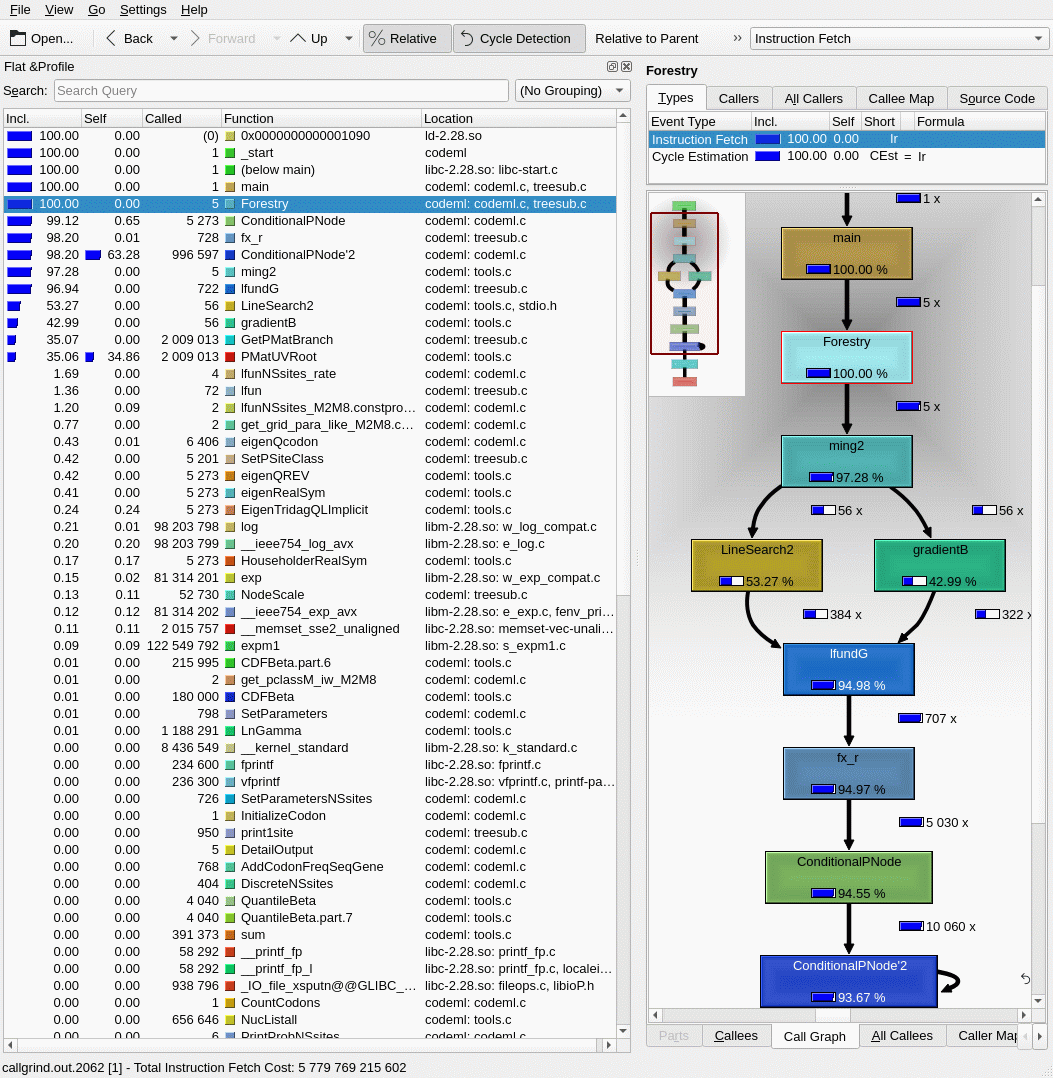
\includegraphics[width=0.3\linewidth]{img/kcachegrind.png} \end{center}
\legend{Fonte: Os Autores} \label{fig:kcachegrind} \end{figure}

\subsection{Implementação}
\label{subsec:codemlpar}

Foi considerada uma implementação paralela para todos os métodos numéricos
supracitados. Em um primeiro momento o cálculo do gradiente foi paralelizado
utilizando OpenMP, um modelo de programação paralela para sistemas com
múltiplos processadores com memória compartilhada.\cite{chandra2001parallel} A
escolha de OpenMP se dá por três fatores: ser adequado ao ambiente de trabalho
dos pesquisadores do HCPA (máquinas multiprocessadas), pela simplicidade de uso
para paralelização de laços, e pela disponibilidade nos ambientes utilizados.

O cálculo do gradiente é aproximado utilizando diferenças finitas para obter as
derivadas parciais de primeiro grau. O codeml permite utilizar diferenças
finitas progressivas, centradas, ou regressivas. A paralelização se dá sob
todas variáveis da função cujo gradiente está sendo obtido. O número de threads
foi definido pelo mínimo entre o número de núcleos de processamento disponíveis
e o número de variáveis na função (iterações no laço). Foi utilizado um
escalonador estático com tamanho do bloco igual ao número de variáveis sob o
número de threads, uma vez que a carga de trabalho é homogênea (as variáveis
são todas da mesma função). O algoritmo encontra-se reproduzido abaixo, onde
$p$ é o número de processadores disponíveis, $t$ o número de threads a ser
usado, $c$ o tamanho do bloco, e $n$ o número de variáveis.

\begin{algorithmic}
\State $t \gets \max(1, \min(p, n))$
\State $c \gets \max(1, \frac{n}{t})$
\For{$i \gets 0,n$ \textbf{in parallel}}
  \If{centrada}
    \State $\frac{\partial f}{\partial x_i} \gets \frac{f(x+h)-f(x-h)}{2h}$
  \ElsIf{progressiva}
    \State $\frac{\partial f}{\partial x_i} \gets \frac{f(x+h)-f(x)}{h}$
  \Else
    \State $\frac{\partial f}{\partial x_i} \gets \frac{f(x)-f(x-h)}{h}$
  \EndIf
\EndFor
\end{algorithmic}

A fim de garantir a corretude da implementação paralela foram desenvolvidos
testes unitários para a função. Em um primeiro momento os testes foram
executados tomando como entrada uma função arbitrária com derivada conhecida,
e os resultados da implementação paralela comparados com aqueles obtidos
simplesmente chamando a função derivada \textit{a priori}. Uma vez que esse
teste foi bem sucedido, testou-se como entrada a função sendo derivada na
implementação do codeml.

Os testes revelaram que a implementação paralela gerava resultados diferentes
da sequencial para a função sendo diferenciada no codeml, mas não para funções
arbitrárias com derivada conhecida. O problema consistia da função sendo
diferenciada ter sido implementada de forma não \textit{thread-safe} pelos
autores do codeml, gerando condições de corrida que inviabilizam a simples
paralelização da rotina em questão.

Foi considerado a reimplementação das funções sendo diferenciadas, todavia, o
uso extensivo de variáveis globais e memória compartilhada na implementação
original do codeml demonstrou-se um grande obstáculo para essa abordagem, que
por isso foi abandonada. Foi estudada então a implementação do slimcodeml, que
reorganiza amplas seções do código fonte, na esperança de que tais
dependências pudessem ter sido removidas, possibilitando a implementação
paralela do cálculo do gradiente. Todavia, apesar de melhor organizado, o
slimcodeml ainda apresenta o mesmo compartilhamento de memória e uso de
variáveis globais encontrados na implementação original, inviabilizando essa
estratégia de paralelização nesse software.

A partir daí foram voltadas as atenções para \textit{LineSearch2}, mas não foi
encontrado na literatura implementações paralelas para o método descrito em
\cite{wolfe1978numerical}, e funções auxiliares utilizadas em seu cálculo
apresentavam os mesmos problemas de compartilhamento de memória encontrados nas
outras rotinas estudadas, tanto na implementação original como no slimcodeml,
portanto a paralelização dessa rotina também foi abandonada.

Por fim, as atenções foram voltadas para o próprio \textit{ming2}, cujo método
numérico (BFGS) é iterativo. Foi realizada uma revisão bibliográfica, que
revelou implementações paralelas desse algoritmo para GPU em
\cite{fei2014parallel}. Os resultados mostram que a implementação não
performa bem para entradas pequenas. Foi realizado então um estudo do uso pelo
codeml desse algoritmo, realizando para isso pequenas adaptações no código para
aumentar a verbosidade dos \textit{logs} da aplicação, ao que observou-se  que
o codeml trabalha com uma entrada fixa de tamanho 61 para esse algoritmo -- o
número códons que traduzem para aminoácidos -- tamanho esse considerado pequeno
com base no estudo supracitado. Dessa forma, conclui-se que uma paralelização
em GPU seria ineficiente. Além disso, a paralelização desse algoritmo é
complexa e de difícil adaptação ao caso do codeml.

Dessa forma, essa abordagem também foi descartada, esgotando todas
possibilidades de paralelização das rotinas responsáveis por quase a totalidade
do tempo de execução do codeml. Ou seja, este trabalho limitou-se à avaliação
de desempenho das alternativas encontradas na literatura, no que tange os
softwares de análise filogenética.

\section{Chamada de variantes: Pacote SAMtools}
\label{sec:SAMtools}

\subsection{Avaliação}

A aplicação samtools providencia o comando \textit{view} para conversão entre
formatos de arquivo, filtragem, e extração de porções de um arquivo, enquanto
comandos como \textit{sort} e \textit{merge} permitem reordenar e agrupar os
arquivos de diversas formas, e os comandos \textit{index} e \textit{faidx}
indexam os arquivos para acesso aleatório rápido. A ferramenta providencia uma
série de outras funcionalidades que fogem ao escopo desse trabalho e estão
descritas em \cite{danecek2021twelve}.

Já a aplicação bcftools, parte do pacote SAMtools, providencia comandos para
execução da chamada de variantes -- \textit{mpileup} e \textit{call}, que
calculam as variantes entre as sequências alinhadas lidas e agrupadas através
de um processo descrito em \cite{li2011improving}. O bcftools providencia mais
21 comandos com mais de 230 opções diferentes para diversas análises das
sequências genéticas alinhadas manipuladas pelo samtools. Uma descrição
completa desses comandos foge ao escopo desse trabalho e pode ser encontrada em
\cite{danecek2021twelve}.

A fim de realizar a chamada de variantes, os pesquisadores primeiro obtém as
sequências genéticas alinhadas de múltiplos indivíduos de pelo menos três
populações no formato CRAM, bem como o genoma de referência no formato FASTA,
descritos na seção \ref{sec:formats}. Todos dados são obtidos do projeto 1000
Genomes.

O fluxo de análise original fornecido pelos pesquisadores pode ser dividido em
três etapas, após a obtenção dos dados. Na primeira etapa é executada uma
conversão de formato de CRAM para BAM utilizando o comando \textit{samtools
view -b}, seguida de uma rotina de indexação dos arquivos utilizando
\textit{samtools index}.

Uma vez convertidos e indexados, cada arquivo de entrada é separado em 22
arquivos de saída, um para cada par de cromossomos autossômicos humanos,
utilizando o comando \textit{samtools view chr}. Essa etapa na sua forma
originalmente usada pelo grupo de pesquisa encontra-se reproduzida na
figura~\ref{fig:stage1_orig}.

\begin{figure}
  \caption{Fluxo de análise original via SAMtools, etapa 1}
    \begin{center}
      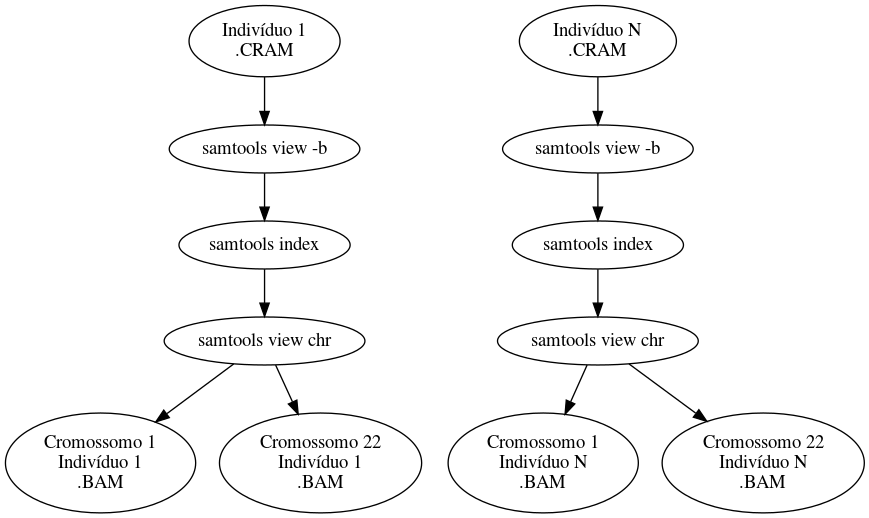
\includegraphics[width=0.85\linewidth]{img/stage1_orig.png}
    \end{center}
    \legend{Fonte: Os Autores}
    \label{fig:stage1_orig}
\end{figure}

Numa segunda etapa, para cada cromossomo são aglutinados os respectivos
arquivos de todos indivíduos, utilizando o comando \textit{samtools merge}.
Posteriormente esses arquivos são indexados, e os comandos \textit{bcftools
mpileup} e \textit{bcftools call} são invocados para executar a chamada de
variantes. O comando \textit{bcftools view} é executado para converter a saída
do formato BCF para VCF, seguido dos comandos \textit{vcftools remove-indels},
que exclui sítios que contenham \textit{indels} (nesse contexto, variantes que
alterem o comprimento do alelo de referência), seguido do comando
\textit{vcftools fiter} para executar um filtro parametrizável por variantes de
interesse. Independente do número de arquivos de entrada, a saída dessa etapa é
sempre 22 arquivos. Ela encontra-se reproduzida na
figura~\ref{fig:stage2_orig}.

\begin{figure}
  \caption{Fluxo de análise original via SAMtools, etapa 2}
    \begin{center}
      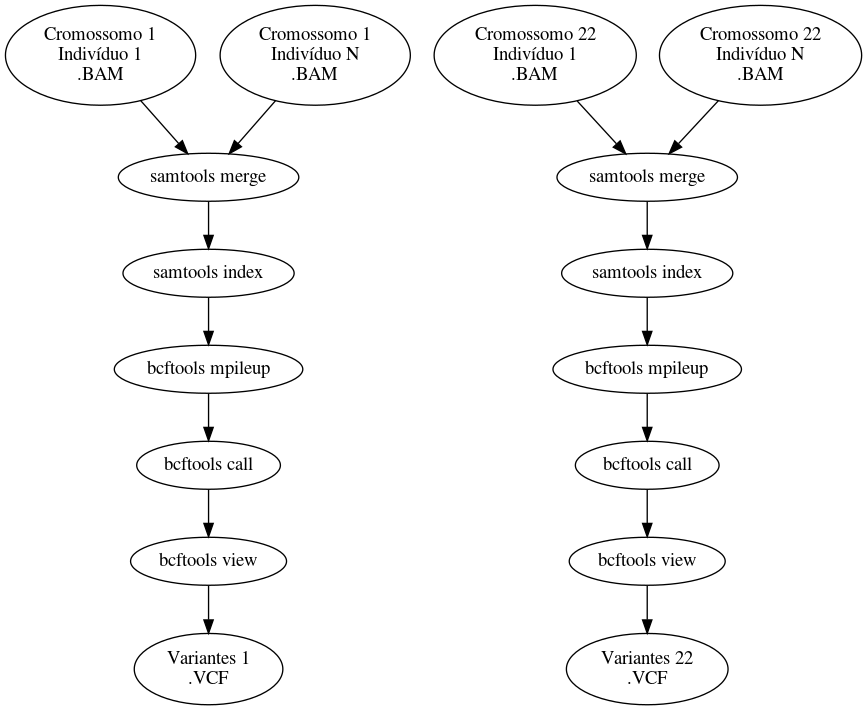
\includegraphics[width=0.85\linewidth]{img/stage2_orig.png}
    \end{center}
    \legend{Fonte: Os Autores}
    \label{fig:stage2_orig}
\end{figure}

A última etapa consiste de concatenar todos arquivos gerados na etapa anterior
utilizando o comando \textit{vcf-concat}, do pacote
VCFtools,\cite{10.1093/bioinformatics/btr330} indexar o arquivo concatenado
utilizando \textit{bcftools index}, e anotar as variantes com a informação
presente no VCF de referência do genoma GRCh38, para isso realizando algumas
conversões de formato via \textit{bcftools view}. Essa etapa recebe sempre 22
arquivos de entrada e produz sempre um único arquivo de saída, e encontra-se
reproduzida na figura \ref{fig:stage3_orig}.

\begin{figure}
  \caption{Fluxo de análise original via SAMtools, etapa 3}
    \begin{center}
      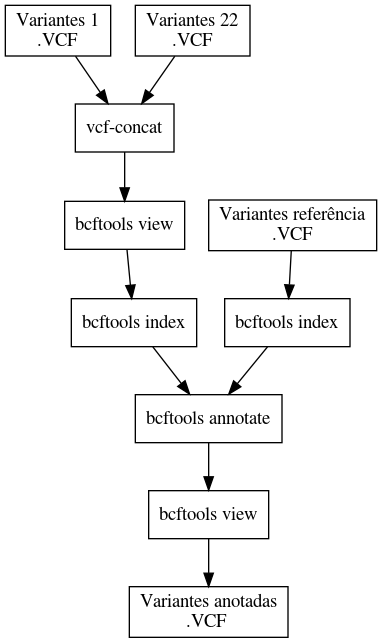
\includegraphics[width=0.85\linewidth]{img/stage3_orig.png}
    \end{center}
    \legend{Fonte: Os Autores}
    \label{fig:stage3_orig}
\end{figure}

Convém ressaltar que os pesquisadores vinham realizando cada uma das etapas
manualmente, porventura repetindo comandos para cada arquivo de entrada ou para
cada cromossomo. Além disso, algumas etapas geram arquivos intermediários que
são necessários somente à etapa posterior, arquivos esses na casa de gigabytes
cada. Isso gerava a necessidade de uma limpeza manual dos arquivos depois de
cada etapa.

\subsection{Benchmark}

Foi realizado um benchmark do tempo de execução de alguns dos comandos
supracitados contra aqueles disponibilizados pela ferramenta sambamba, descrita
em \ref{sec:SAMtools}, a fim avaliar seu uso como alternativa. Os resultados
encontram-se descritos abaixo.

A conversão de CRAM para BAM para uso do sambamba foi realizada usando o
samtools, uma vez que o sambamba, apesar de providenciar tal suporte em suas
versões mais antigas, apresentou problemas na leitura dos arquivos -- no
\textit{issue tracker} do projeto há relatos desses problemas, e a resposta dos
autores foi remover o suporte a CRAM completamente. Cada conversão leva entre
duas e três horas para arquivos de entrada entre 22 GB e 34 GB, na máquina
Thor1, cujo hardware está descrito na tabela \ref{tbl:thor1}.

Feita a conversão, foram testados individualmente os comandos providenciados
pela ferramenta sambamba, comparando com os comandos equivalentes da ferramenta
samtools. O comando de indexação foi consideravelmente mais lento na ferramenta
sambamba, apesar de usar múltiplos núcleos enquanto o samtools roda
sequencialmente. Enquanto o samtools levou 39s para indexar um CRAM de 26 GB, o
sambamba levou 2m 9s para indexar o BAM convertido a partir dele, de 53 GB. A
amostra utilizada foi a HGDP00519.

Já para a rotina de visualização de uma região ou cromossomo o sambamba foi
consideravelmente mais rápido. Enquanto o samtools levou 4m 5s para visualizar
uma região do arquivo supracitado, o sambamba levou apenas 19s. Já os comandos
de \textit{merge} e \textit{mpileup} não puderam ser executados com o sambamba
-- para o mesmo arquivo em que os comandos mencionados anteriormente rodaram
com sucesso, tais comandos apresentaram erros sobre o formato do arquivo, tanto
na versão mais atual do sambamba como em versões anteriores. A tabela
\ref{tbl:sambamba} sumariza os resultados.

\begin{table}[h]
  \caption{\textit{Benchmark} da ferramenta sambamba}
    \centering
        \begin{tabular}{c|c|c}
          \hline
          \textit{Comando}  &   \textit{Tempo samtools}  & \textit{Tempo sambamba} \\
          \hline
          \hline
          view (convert) & 2h 41m & N/A \\
          index & 39s & 2m 9s \\
          view region & 4m 5s & 19s \\
          merge & 8m & N/A \\
          pileup & 1h 3m & N/A \\
          \hline
        \end{tabular}
      \legend{Fonte: Os autores}
    \label{tbl:sambamba}
\end{table}

Observa-se que os resultados não são diretamente comparáveis com aqueles
apresentados em \cite{tarasov2015sambamba}, visto que lá os autores utilizam
arquivos BAM com o SAMtools, enquanto que neste trabalho são utilizados
arquivos CRAM, significativamente menores. Diante desses resultados optou-se
por não utilizar o sambamba. O único cenário em que seu uso seria benéfico é na
visualização das regiões, mas como o sambamba não trabalha com CRAM seria
necessário uma conversão custosa, de várias horas para cada arquivo de entrada,
para uma redução no tempo de execução de poucos minutos para alguns segundos.
No total, não traria benefícios aos usuários.

\subsection{Perfil de execução}

Através de um estudo da literatura e do manual das ferramentas utilizadas
percebeu-se oportunidade de melhorias no fluxo de análise utilizado pelos
pesquisadores. Em particular, em \cite{danecek2021twelve} os autores observam
que o uso do comando \textit{samtools view -b}, para conversão de CRAM para
BAM, apesar de frequentemente presente em guias na internet é normalmente
desnecessário, uma vez que as ferramentas possuem suporte a CRAM. Isso ocorre
por motivos históricos, pois originalmente o SAMtools não trabalhava com
arquivos CRAM.\cite{danecek2021twelve}

Foi medido o tempo de execução de cada um dos comandos que compõem o fluxo
original de análise, expostos na tabela \ref{tbl:sambamba}, para uma entrada
de uma amostra. A conversão de CRAM para BAM era particularmente custosa.
Observado isso, foi testado e comprovado que todo restante da análise poderia
ser executado sem essa etapa, observando o suporte para CRAM e comparando as
saídas do fluxo otimizado com o fluxo original. Dessa forma, essa etapa de
conversão foi removida no fluxo otimizado.
P
Ainda em \cite{danecek2021twelve} os autores comentam que conversões de BCF
para VCF são custosas e porventura desnecessárias. Na última etapa do fluxo de
análise original é realizada tal conversão seguida de um filtro, para uso dos
arquivos pela ferramenta VCFtools. Apesar do nome, essa ferramenta também
trabalha com arquivos no formato BCF.\cite{man2015vcftools} Foi experimentada a
remoção da etapa de conversão supracitada, substituindo o filtro com o
utilitário \textit{vcfutils} do pacote SAMtools pela filtragem com o próprio
bcftools utilizando o comando \textit{filter}. Com isso foi observado que a
maior parte do tempo de execução está na filtragem e não na conversão, e não
houve diferença significativa de desempenho do VCFtools usando BCF ou VCF. Por
fim, os pesquisadores precisam dos arquivos de saída finais no formato VCF para
análise estatística dos dados em texto plano, portanto uma conversão é
inevitável. Dessa forma, diferente da conversão de CRAM para BAM, a conversão
de BCF para VCF foi mantida no fluxo otimizado.

Na última etapa do fluxo original estava presente uma etapa de indexação das
variantes do genoma de referência, sendo uma etapa custosa, visto que o arquivo
sendo indexado possui 15 GB comprimido, precisa ser descomprimido e depois
indexado. Todavia, o mesmo projeto (NCBI) que fornece o arquivo das variantes
do genoma de referência também fornece o respectivo arquivo de índice, que tem
apenas 2,7 megabytes. Dessa forma, a etapa de indexação foi substituída pelo
download do índice de referência, novamente economizando tempo de execução.

\subsection{Implementação}

Foi observado ainda que as duas primeiras etapas do fluxo original eram
embaraçosamente paralelas, consistindo de passos independentes para cada
arquivo de entrada.  Como os pesquisadores do HCPA possuem acesso a máquinas
multiprocessadas, foi realizada uma paralelização de ambas etapas utilizado GNU
Parallel\cite{tange_ole_2021_5233953}. A escolha dessa ferramenta se deu pela
facilidade de uso, disponibilidade nos ambientes usados pelos pesquisadores, e
suporte a ajuste automático do número de \textit{jobs} paralelos ao número de
núcleos de processamento disponíveis. Foi desenvolvida uma ferramenta para
execução do fluxo de análise otimizado e paralelizado. Um pseudo código da
ferramenta encontra-se reproduzido abaixo.

\begin{algorithmic}
  \State $C \gets \text{input CRAMs}$
  \State $n \gets \text{input length}$
\For{$j \gets 0,n$ \textbf{in parallel}}
  \State samtools index C(j)
  \For{$i \gets 1,22$}
    \State $R(i,j) \gets \text{samtools view } C(j) \text{ chr i}$
  \EndFor
\EndFor

\For{$i \gets 1,22$ \textbf{in parallel}}
  \State $M(i) \gets \text{samtools merge } R(i,j)$ \textbf{for j in 0,n}
  \State samtools index $M(i)$
  \State bcftools mpileup $M(i)$
  \State bcftools call $M(i)$
  \State bcftools view $M(i)$
  \State vcftools remove-indels $M(i)$
  \State vcftools filter $M(i)$
\EndFor

\State $C \gets \text{vcf-concat } M(i)$ \textbf{for i in 1,22}
\State bcftools view C
\State bcftools index C
\State bcftools annotate C
\State bcftools view C
\end{algorithmic}

A validação da corretude das ferramentas se deu através da comparação das
saídas do pipeline original e otimizado, validando tais resultados junto aos
pesquisadores do HCPA.

Validada a corretude da implementação, foram realizados novos benchmarks de seu
tempo de execução. As otimizações e a paralelização reduziram drasticamente o
tempo de análise. Na tabela \ref{tbl:SAMtools} encontram-se reproduzidos os
tempos de execução utilizando o pipeline original e o otimizado. Os testes
foram realizados na máquina Thor1, descrita na tabela \ref{tbl:thor1},
utilizando todos núcleos de processamento disponíveis. Foram utilizados como
entrada as amostras HGDP00715, HGDP00711, HGDP00519, HGDP00714, HGDP00712,
HGDP00777, HGDP00525, e HGDP00719.

\begin{table}[h]
    \caption{Tempos de execução do SAMtools}
    \centering
        \begin{tabular}{c|c|c}
          \hline
          \textit{Tamanho da entrada}  &   \textit{Tempo original}  & \textit{Tempo otimizado} \\
          \hline
          \hline
          58 GB (2 CRAMs) & 1d 4h 55m & 4h 59m \\
          124 GB (4 CRAMs) & 2d 9h 50m & 7h 39m \\
          232 GB (8 CRAMs) & 4d 14h 35m & 12h 8m \\
          \hline
        \end{tabular}
      \legend{Fonte: Os autores}
    \label{tbl:SAMtools}
\end{table}

Além disso, foram realizados testes de desempenho para entradas com 2 arquivos
(58 GB) e 6 arquivos (161 GB) utilizando um número diferente de núcleos de
processamento, a fim de estimar o speedup bem como a quantidade de
tempo economizado pela paralelização, o resto sendo atribuído às otimizações no
fluxo de análise. Os resultados encontram-se reproduzidos nas tabelas
\ref{tbl:speedup2} e \ref{tbl:speedup6}.

\begin{table}[h]
    \caption{Speedup da ferramenta com duas entradas}
    \centering
        \begin{tabular}{c|c|c}
          \hline
          \textit{Número de núcleos}  &   \textit{Tempo de execução}  & \textit{Speedup} \\
          \hline
          \hline
          1 núcleo & 20h 26m & N/A \\
          2 núcleos & 10h 46m & 1.90x \\
          4 núcleos & 6h 12m & 3.29x \\
          6 núcleos & 4h 59m & 4.10x \\
          \hline
        \end{tabular}
      \legend{Fonte: Os autores}
    \label{tbl:speedup2}
\end{table}

\begin{table}[h]
    \caption{Speedup da ferramenta com seis entradas}
    \centering
        \begin{tabular}{c|c|c}
          \hline
          \textit{Número de núcleos}  &   \textit{Tempo de execução}  & \textit{Speedup} \\
          \hline
          \hline
          1 núcleo & 2d 1h 33m & N/A \\
          2 núcleos & 1d 58m & 1.98x \\
          4 núcleos & 13h 16m & 3.73x \\
          6 núcleos & 9h 30m & 5.22x \\
          \hline
        \end{tabular}
      \legend{Fonte: Os autores}
    \label{tbl:speedup6}
\end{table}

\begin{table}[h]
    \caption{Tempos de execução da ferramenta por etapa}
    \centering
        \begin{tabular}{c|c|c|c|c}
          \hline
          \textit{Entradas}  & \textit{Núcleos} & \textit{Etapa 1}  & \textit{Etapa 2} & \textit{Etapa 3} \\
          \hline
          \hline
          2 CRAMs & 1 núcleo  & 1h 44m &    18h 21m & 21m \\
          2 CRAMs & 2 núcleos &    59m &     9h 26m & 21m \\
          2 CRAMs & 4 núcleos & 1h     &     4h 52m & 20m \\
          2 CRAMs & 6 núcleos & 1h     &     3h 38m & 21m \\
          6 CRAMs & 1 núcleo  & 4h 12m & 1d 21h  2m & 20m \\
          6 CRAMs & 2 núcleos & 2h 41m &    21h 55m & 22m \\
          6 CRAMs & 4 núcleos & 1h 40m &    11h 15m & 21m \\
          6 CRAMs & 6 núcleos & 1h 04m &     8h  6m & 20m \\
          \hline
        \end{tabular}
      \legend{Fonte: Os autores}
    \label{tbl:stages}
\end{table}

O speedup para duas entradas é menor do que o ideal, tão menor quanto maior o
número de núcleos utilizados. Isso é esperado, uma vez que não estamos
utilizando todos núcleos disponíveis na etapa 1 quando há somente duas
entradas. Para seis entradas o mesmo é observado, mas o speedup fica mais
próximo do ideal. Isso é esperado, visto que utilizamos todos núcleos
disponíveis em todas etapas, exceto a última.

Conforme pode ser observado na tabela \ref{tbl:stages}, que discrimina os
resultados por etapa, o maior ganho com o paralelismo está na etapa 2, em que é
lançado um \textit{job} para cada um dos 22 cromossomos, limitado ao número de
CPUs disponíveis. Conforme esperado, a etapa 1, em que é lançado um
\textit{job} para cada entrada, limitado pelo número de CPUs disponíveis, só
tem ganho de desempenho até o número de \textit{jobs} ser igual ao número de
entradas. Por fim, conforme esperado, a etapa 3 tem tempo constante, uma vez
que executa em uma única thread -- mas possui ganho de desempenho em relação ao
pipeline original em que havia uma etapa de indexação desnecessária.

Observa-se que uma alternativa à paralelizar somente os \textit{jobs} sob cada
entrada seria utilizar um pipeline dos comandos, dado que, para alguns
comandos, a saída de um é a entrada do seguinte. Dessa forma, ambos poderiam
ser executados em paralelo de forma que a saída fosse consumida assim que
gerada. Esse IO poderia ser feito ainda em memória volátil, reduzindo as
escritas e leituras em disco. Um mecanismo para realizar essa tarefa de
comunicação entre processos (IPC) seria pipes POSIX, que fornecem uma interface
simples para direcionar a saída de um programa à entrada do próximo, ambos
rodando em paralelo, usando um buffer em memória volátil para
isso.\cite{immich2003performance} Num ambiente POSIX, pipes são também a
escolha com melhor desempenho para IPC.\cite{immich2003performance}

Todavia, o fato do IO residir em memória volátil incorre em uso mais elevado
desse recurso, justamente o que tentava-se evitar ao buscar uma alternativa a
softwares como ANGSD e PVCtools. Dessa forma, uma vez testado e observado que o
uso de memória tornava-se elevado demais utilizando um pipeline, foi mantida
somente a paralelização de \textit{jobs} sob os arquivos de entrada, com
remoção automática dos arquivos intermediários gerados por cada etapa, operação
antes realizada manualmente pelos pesquisadores. Observa-se que é precisamente
esse tipo de abordagem que tomam os softwares sambamba e elPrep, que apresentam
uso de memória demasiadamente elevado.

Tanto o samtools como o bcftools e a ferramenta desenvolvida pelos autores
requerem um ambiente com uma série de softwares pré-instalados e em versões
específicas, o que porventura gerava dificuldades aos pesquisadores do HCPA. A
fim de superar tais dificuldades decidiu-se por utilizar o software Docker,
também utilizado nas análises de desempenho. Além disso, foi desenvolvida uma
interface gráfica para o uso do samtools e bcftools para chamada de variantes.
O intuito é facilitar o uso do ferramental para profissionais da biologia que
porventura não estejam familiarizados com interfaces por linha de comando.

A interface é executada na máquina local do usuário, que pode configurar uma
máquina remota para execução do pipeline de análise. Além da execução do
pipeline, a interface automatiza uma série de outros passos realizados pelos
pesquisadores, como obtenção dos dados e manipulação dos arquivos de resultado.
A interface permite ainda realizar todas etapas em segundo plano, verificar seu
progresso, e interrompê-las.

Para desenvolvimento da interface optou-se por utilizar a linguagem de
programação Python, amplamente utilizada para computação
científica.\cite{oliphant2007python} A escolha da linguagem se deu
principalmente pelo sua disponibilidade em múltiplos sistemas operacionais,
visto que os usuários (pesquisadores do HCPA) manifestaram interesse em
utilizar a ferramenta nos sistemas operacionais Windows, Linux, e Mac, e há
suporte tanto de interpretadores da linguagem como das bibliotecas utilizadas
para todas essas plataformas.\cite{oliphant2007python} Outro fator que
influenciou a escolha foi a agilidade no desenvolvimento que a linguagem
proporciona.\cite{oliphant2007python}

Foi utilizada a biblioteca \textit{guietta} para criação da interface
gráfica,\cite{guietta} um \textit{wrapper} em cima da biblioteca
\textit{PySide2}, um \textit{binding} para Python da biblioteca multiplataforma
Qt.\cite{loganathan2013pyside} A escolha da biblioteca vem pela sua facilidade
de uso e pela disponibilidade multiplataforma. As figuras
\ref{fig:samgui_linux}, \ref{fig:samgui_mac}, e \ref{fig:samgui_windows}
apresentam uma captura de tela da interface gráfica desenvolvida nas
plataformas Linux, Mac, e Windows, respectivamente.

\begin{figure}
  \caption{Captura de tela da interface gráfica ``SAMGUI'' em ambiente Linux}
    \begin{center}
      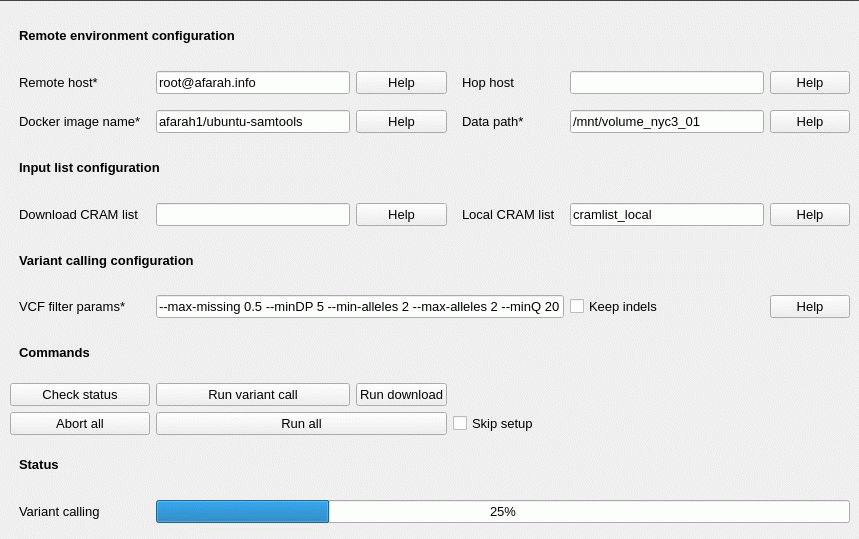
\includegraphics[width=0.85\linewidth]{img/samgui_linux.png}
    \end{center}
    \legend{Fonte: Os Autores}
    \label{fig:samgui_linux}
\end{figure}

\begin{figure}
  \caption{Captura de tela da interface gráfica ``SAMGUI'' em ambiente Mac}
    \begin{center}
      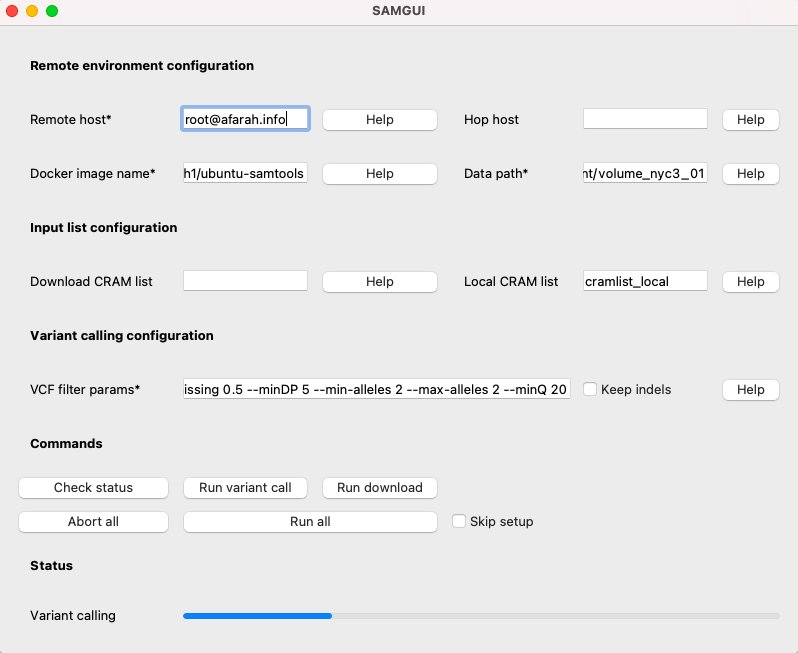
\includegraphics[width=0.85\linewidth]{img/samgui_mac.png}
    \end{center}
    \legend{Fonte: Os Autores}
    \label{fig:samgui_mac}
\end{figure}

\begin{figure}
  \caption{Captura de tela da interface gráfica ``SAMGUI'' em ambiente Windows}
    \begin{center}
      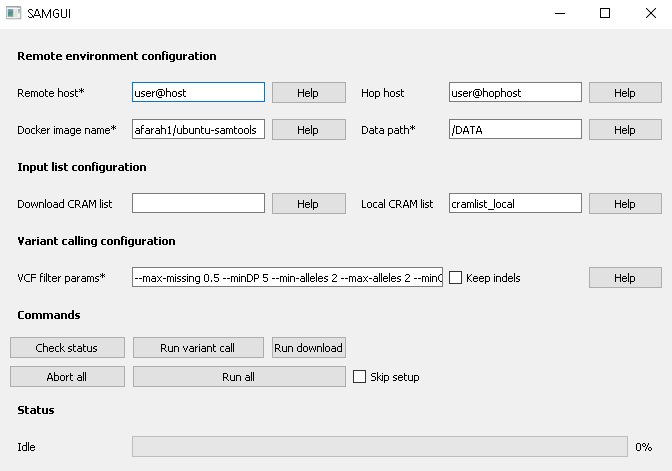
\includegraphics[width=0.85\linewidth]{img/samgui_windows.png}
    \end{center}
    \legend{Fonte: Os Autores}
    \label{fig:samgui_windows}
\end{figure}

\section{Chamada de variantes: Pacote ANGSD}
\label{sec:angsd}

\subsection{Avaliação}

Outra aplicação utilizada pelo grupo de pesquisa em genética é o pacote ANGSD,
software para análise genética de diferentes populações de uma
espécie.\cite{korneliussen2014angsd} Os pesquisadores utilizam esse software
para determinar se a genética de uma população influencia em alguma
característica específica de seus indivíduos, através de um teste chamado
\textit{Population Branch Statistic} (PBS), caracterizado pela comparação da
frequência de ocorrência de determinados alelos entre pares de
indivíduos de diferentes populações.\cite{yi2010sequencing}

A análise em questão consiste de duas etapas, a primeira utilizando o binário
angsd, a aplicação principal do pacote ANGSD, e a segunda etapa utilizando a
ferramenta realSFS, um utilitário fornecido pelo pacote. A primeira etapa leva
cerca de um dia para cada arquivo de entrada e porventura apresenta uso elevado
de memória, enquanto que a segunda etapa, que recebe como entrada a saída da
etapa anterior, nunca termina a execução devido a uso de memória
proibitivamente elevado, para os dados de entrada dos pesquisadores do HCPA.

A entrada da primeira etapa consiste em arquivos nos formatos BAM ou CRAM,
descritos na seção \ref{sec:formats}, um arquivo de entrada para cada indivíduo
de cada população sob análise. O angsd então utiliza a biblioteca
htslib para manipulação desses arquivos.

Uma primeira observação realizada através de reuniões com os pesquisadores é
que esses dados de entrada são obtidos sempre no formato CRAM do projeto 1000
Genomes, e que estava sendo realizada uma etapa de conversão de CRAM para BAM
para uso do angsd. Essa conversão é realizada utilizando o software SAMtools,
descrito em mais detalhes na seção \ref{sec:SAMtools}, e leva algumas horas
para cada arquivo de entrada. Todavia, como observado anteriormente, o angsd
trabalha também com o formato CRAM, fato esse observado através do estudo do
manual da ferramenta. Sendo assim, a etapa de conversão é desnecessária. Essa
observação já economizou algumas horas de execução.

Eliminada essa etapa de pré-processamento dos dados, realizou-se um perfil de
execução do software a fim de elucidar seu alto uso de memória. Foi utilizada a
ferramenta massif, do software valgrind.

\subsection{Perfil de execução}

Inicialmente realizou-se um estudo do utilitário realSFS, que apresentava o
principal problema de desempenho. Através de um estudo do código fonte foi
observado que o utilitário implementa dois otimizadores, um legado utilizando
BFGS (o mesmo algoritmo usado no pacote PAML) e o padrão utilizando
``Electromagnetism-like Mechanism'', um método estocástico de otimização
não linear que utiliza mecanismos de atração e repulsão para mover
''partículas`` na direção ótima.\cite{5636954} Foi observado ainda que,
independente do otimizador utilizado, a alocação de memória é a mesma. Fatores
que influenciam no uso de memória incluem o número de threads e o número de
sítios considerados. Em ambos os casos há um \textit{trade-off} - ao reduzir o
número de threads o tempo de execução aumenta, e ao reduzir o número de sítios
a confiabilidade dos resultados diminui.\cite{popgen2016angsd} A redução de
ambos é indesejável, visto que o tempo de execução já é muito elevado e a
confiabilidade dos resultados é fundamental.

Foi traçado então um perfil de memória da aplicação utilizando massif,
visando elucidar as causas do uso elevado de memória. Esse perfil revelou que a
etapa de otimização supracitada é o principal responsável pelo uso
proibitivamente alto de recursos, e não foram encontradas oportunidades de
melhoria que não afetassem o tempo de execução ou a confiabilidade dos
resultados.

Foi realizada uma reunião com os pesquisadores, em que foi observado que é
possível realizar a mesma análise feita com o angsd (PBS) utilizando o pacote
SAMtools, construído em cima da biblioteca htslib (tal qual o angsd), e que já
era utilizado na etapa de pré-processamento dos dados, seguida de uma análise
estatística dos resultados. Todavia, o pipeline de análise utilizando tais
ferramentas apresentava tempos proibitivamente lentos. Na seção
\ref{sec:SAMtools} é descrito um estudo desse pipeline e o posterior
desenvolvimento de uma ferramenta que otimiza e paraleliza sua execução,
resolvendo o problema de desempenho supracitado. Tal estudo foi realizado em
paralelo ao estudo do angsd descrito acima e, uma vez que os resultados foram
se mostrando mais frutíferos, o foco dese trabalho passou a ser esse
ferramental, a análise pelo angsd sendo substituída pela análise pelo SAMtools
por parte dos pesquisadores.

%
%
% Conclusão
%
%
\chapter{Conclusão}
\label{chap:conc}

Neste trabalho foram estudados os softwares de bioinformática usados pelos
pesquisadores do Hospital de Clínicas de Porto Alegre, nomeadamente os
softwares de análise filogenética e chamada de variantes, com um foco nos
pacotes PAML e SAMtools, que realizam tais tarefas, respectivamente.

No caso dos softwares de análise filogenética foi realizado um estudo da
literatura, análise de desempenho das soluções encontradas e da solução de
referência usada pelos pesquisadores do HCPA (pacote PAML), além de uma
tentativa de paralelização do software original. Com isso, concluiu-se que uma
implementação paralela exigiria grande esforço, provavelmente necessitando uma
reescrita do software para eliminar compartilhamento de memória e uso
abundante de variáveis globais presentes na implementação original que
dificultam sua paralelização. Além disso, foi encontrada solução na literatura
que reduz em mais da metade o tempo de processamento para o caso de uso dos
pesquisadores do HCPA, sendo essa a alternativa adotada para análise
filogenética.

Para os softwares de chamada de variantes também foi realizado uma revisão
bibliográfica e análises de desempenho, além do desenvolvimento de uma
ferramenta própria que paraleliza \textit{jobs} da aplicação de referência
(SAMtools), otimizando o pipeline de chamada de variantes utilizado até então
pelos pesquisadores do HCPA, além de fornecer uma interface gráfica para sua
operação. A escolha de desenvolvimento de uma solução própria que paraleliza
\textit{jobs} da aplicação de referência visa superar deficiências presentes em
soluções encontradas na literatura, nomeadamente o uso elevado de memória, a
ausência de suporte ao formato de arquivo CRAM utilizado pelo projeto 1000
Genomes, e o uso de implementações próprias sem testes extensivos.

Foram realizados testes de desempenho comparando a ferramenta desenvolvida
nesse trabalho com aquelas encontradas na literatura, a ferramenta desenvolvida
pelos autores apresentando uma série de vantagens. Nomeadamente, o uso de
memória foi significativamente inferior àquele das ferramentas ANGSD e
PVCtools, e o uso da implementação da referência (SAMtools) confere maior
confiabilidade à ferramenta versus implementações próprias como no caso da
sambamba, além de suporte a arquivos CRAM. Ao mesmo tempo, a ferramenta
apresenta tempo de execução superior ao uso sequencial da implementação de
referência, e a ausência de necessidade de conversão de CRAM para BAM torna-a
superior em alguns aspectos às ferramentas sambamba e elPrep, sendo uma
alternativa de paralelização de chamada de variantes. Por fim, a
disponibilização de uma interface gráfica facilita o uso por profissionais não
familiarizados com interfaces de linha de comando, e o uso de containers Docker
facilita a reprodução dos resultados obtidos nesse trabalho.

\section{Discussão e trabalho futuro}

Além do pacote SAMtools e softwares alternativos a ele, existem diversas
ferramentas utilizados para chamadas de variante utilizando modelos diferentes
daquele empregado pelo SAMtools, produzindo resultados discrepantes conforme
descrito na seção \ref{sec:alt}.

Um trabalho futuro consiste em explorar o uso dessas ferramentas junto aos
pesquisadores do grupo de pesquisa em genética, com avaliação tanto de seu
desempenho como da aplicabilidade desse ferramental considerando os resultados
potencialmente diferentes entre si, para o caso de uso do HCPA, levando em
consideração a literatura a respeito dessas ferramentas.

Outra linha de trabalho futuro é a adição de suporte a arquivos CRAM às
ferramentas sambamba e elPrep, a fim de adequá-las aos arquivos atualmente
disponibilizados pelo projeto 1000 Genomes. Uma abordagem seria utilizar a
htslib para isso, levando em consideração que essas ferramentas dividem os
arquivos de entrada para processamento -- não bastaria simplesmente utilizar a
API para leitura do arquivo CRAM completo para memória.

Por fim, outro trabalho futuro consiste no estudo de uma abordagem para cluster
e comparação com as ferramentas presentes na literatura que adotam tal
abordagem. Um desafio em tal abordagem é a transferência dos dados entre os
nodos de execução, uma vez que cada etapa intermediária produz saídas de vários
gigabytes para cada entrada. Uma possibilidade é o uso de frameworks Apache
Flink, especificamente projetado para processamento paralelo e com tolerância a
falhas de pipelines (isto é, fluxos de execução em que a entrada de uma etapa é
a saída da anterior).\cite{carbone2015apache}

%
%
% Referências
%
%

\bibliographystyle{abntex2-alf}
\bibliography{biblio}

\end{document}
